\chapter{运行设计}

\section{系统启动流程}
系统在冷启动及后续运行时，前端单页面应用首先通过边缘托管节点将打包好的轻量静态资源分发给用户浏览器。用户浏览器在首屏加载完成后，自动触发首行代码中的鉴权探测机制，即尝试从本地 \texttt{localStorage} 中拉取用户的 JWT 令牌。

如果检测到令牌缺失，前端子系统将自动重定向至登录与注册页面；如果令牌存在，前端将携带此令牌向后端 \texttt{/users/me} 路由发起安全身份验证请求。后端验证签名无误后，返回封装好的 \texttt{UserDto} 用户角色，前端上下文状态机随之激活并根据该角色加载专属侧边工作台导航。此启动流程全部在浏览器本地与服务器节点之间以异步非阻塞方式进行，实现了无状态的快速启动。

\section{核心业务运行流程}
系统最具代表性的核心业务是虚拟互动课堂的编排与授课全链路闭环。

业务始于教师在“课程信息 (Info)”和“排课表 (Schedule)”面板中新建课时节点，设定起始和结束时间，并在“课件管理 (Courseware)”中上传 PDF 课件。在上传课件时，系统支持将特定文件标为课时或课程级别的默认课件，并将其唯一标识持久化为 \texttt{defaultCoursewareFileId}，从而在数据库大纲中建立关联。

当学生在日程看板或个人主页上检测到所属课程的直播即将开始并点击进入教室时，系统将动态触发学生等待室机制。如果此时授课教师尚未进入教室建立信道，学生端会进入等待状态，并且前端信令模块会自动在后台以自适应指数退避策略对后端的 Presence 信道执行无声轮询。

一旦教师点击“进入教室”，教师端浏览器会迅速与部署在服务器上的 WebSocket 在线服务建立长连接信道。此时，后端 Presence 心跳中心即刻被点亮并自动检测该课时的 \texttt{defaultCoursewareFileId}。若存在关联的默认课件，后端会将课件文件标识和当前默认的第 1 页页码组装为同步控制信令，向所有处于指数退避等待状态的学生端广播。

学生端前台接收到此信令后，结束等待状态，在浏览器本地调用 PDF.js 对默认课件进行 Canvas 绘制。在随后的教学过程中，教师在界面上进行翻页或标记时，位置与页码数据会以紧凑的二进制帧封装，通过 WebSocket 信道广播给全体学生，实现同步交互授课。

虚拟互动课堂启动及学生端指数退避自愈轮询活动逻辑流程如图 6.2 所示。

\begin{figure}[H]
\centering
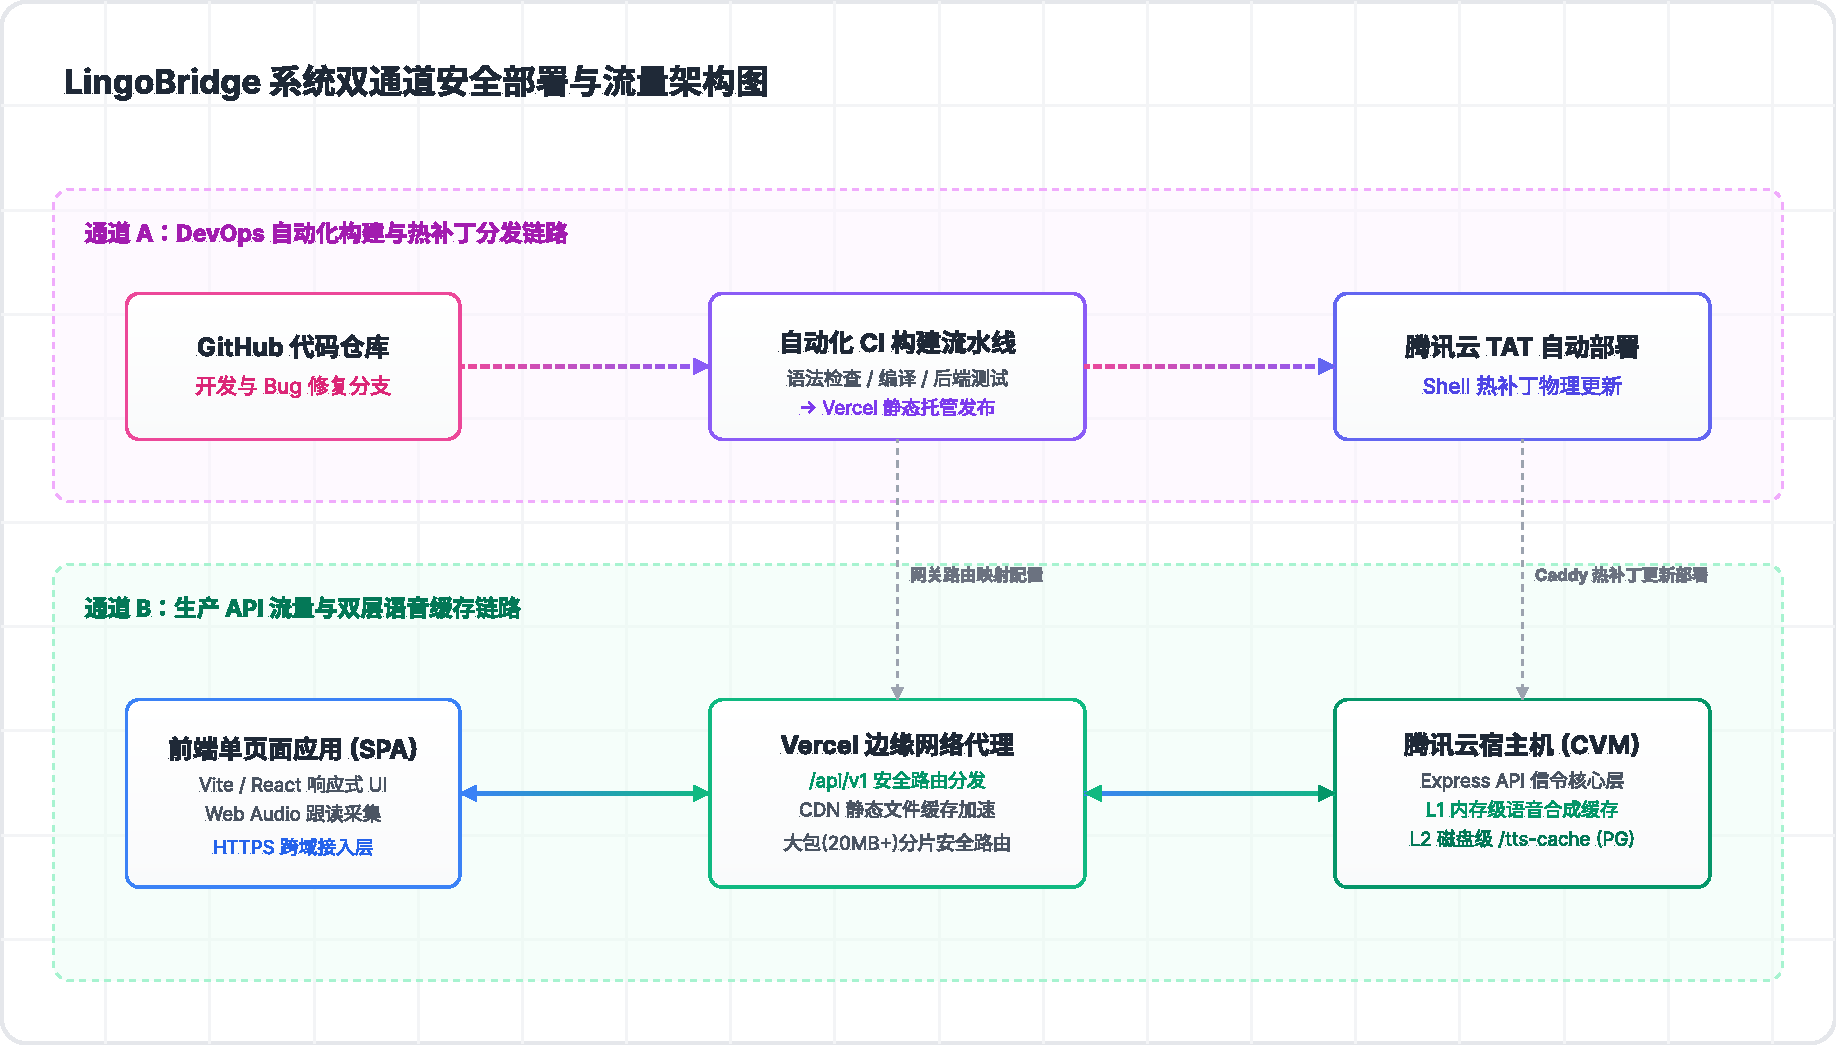
\includegraphics[width=0.68\textwidth]{figures/runtime-activity.pdf}
\caption{LingoBridge 虚拟课堂启动及指数退避自愈轮询活动图}
\label{fig:runtime_activity}
\end{figure}


\section{任务调度与并发处理}
后端服务层基于 Node.js 经典的非阻塞单线程事件循环架构运行。为了应对直播课堂中可能出现的并发翻页以及心跳信令，系统底层避开了多线程阻塞式连接，而是通过高内聚的异步 I/O 事件回调实现极速流转。

当高频的 WebSocket 心跳及在线状态探测请求抵达服务器时，操作系统的反向代理层首先会将其复用，由后端的 Express 事件环单线程在内存中进行微毫秒级的 Presence 数据字典状态更新。所有的物理磁盘 I/O（如录音文件缓冲写入、备份脚本执行等）均被抛入操作系统的内核异步线程池中并行处理。这种节约计算资源、通过轻量级异步信道进行任务分发的设计，确保了平台即使在极轻量云服务器环境下，也能稳健承载试点学校的小班在线授课并发。

\section{系统状态转换设计}
系统交互的核心机制是通过后端的 Presence 状态机来调度课堂生命周期的流转。LingoBridge 在线虚拟教室 Presence 状态转换图如图 6.1 所示。

\begin{figure}[H]
\centering
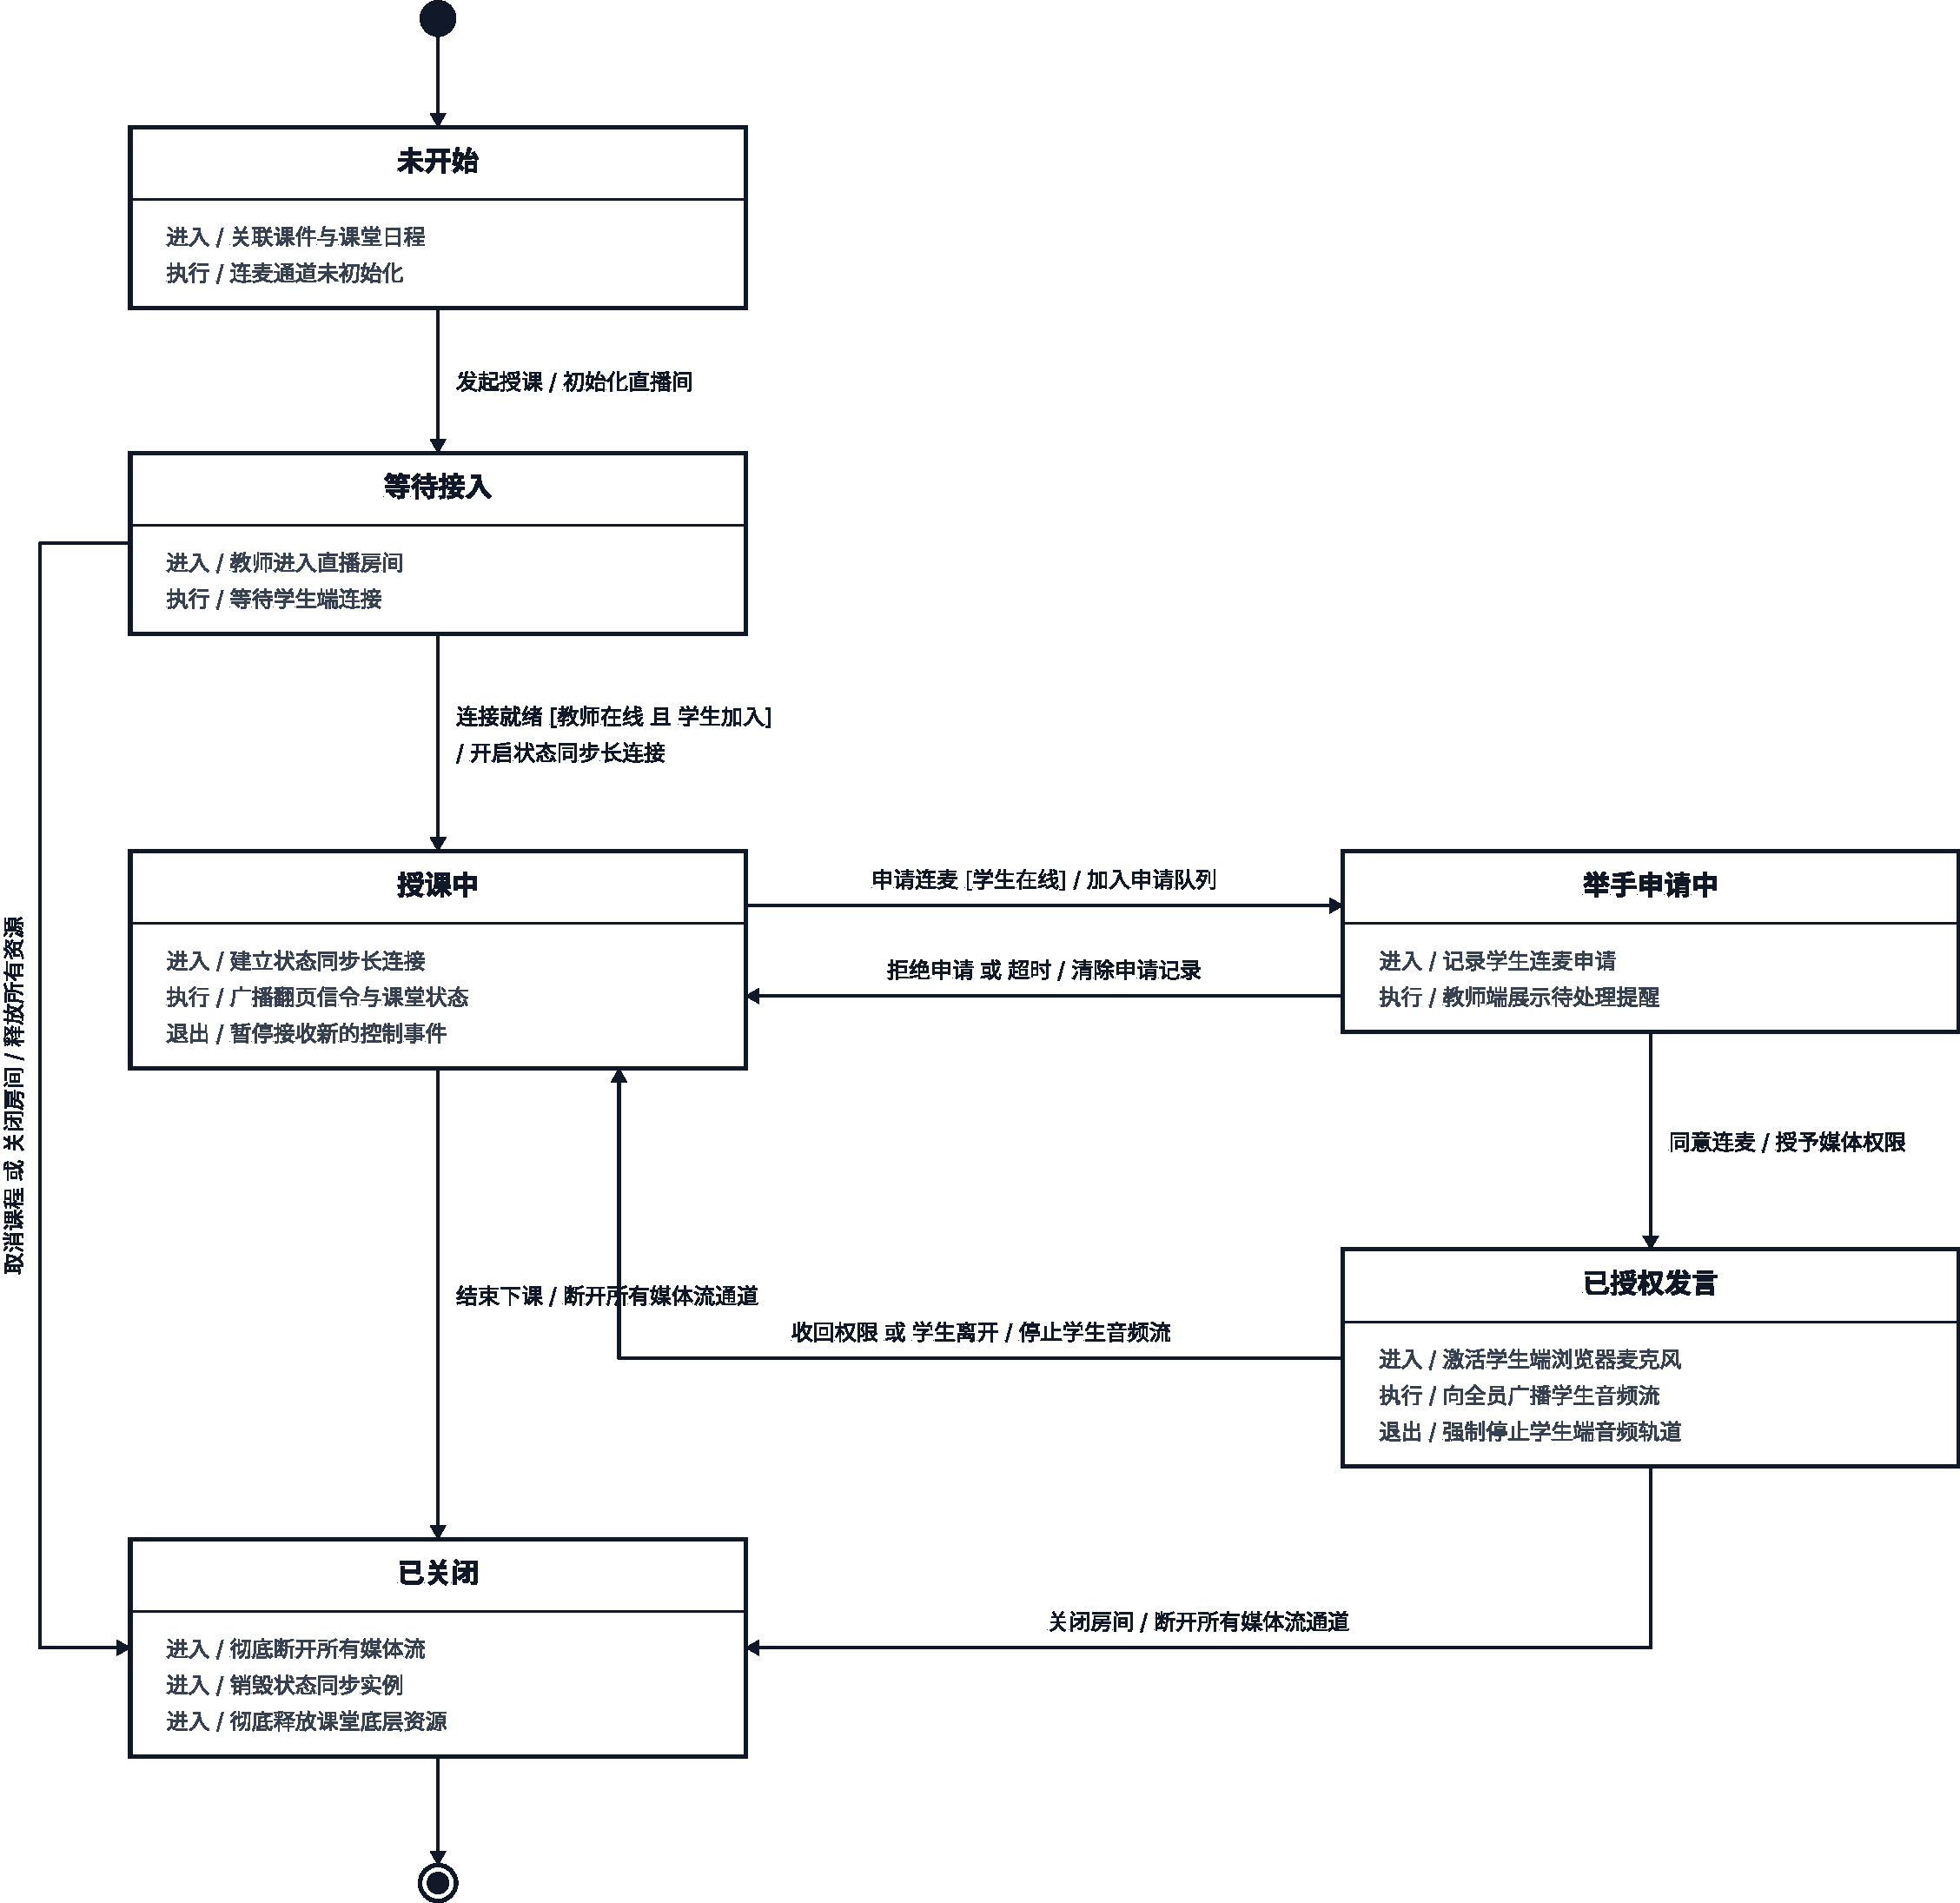
\includegraphics[width=0.72\textwidth]{figures/LingoBridge状态图.pdf}
\caption{LingoBridge 虚拟课堂 Presence 状态转换图}
\label{fig:state_main}
\end{figure}

如图 6.1 所示，课时生命周期由空闲（\texttt{idle}）状态开启，即课时已排定但无用户进入。当教师进入并与信令中心握手成功后，状态即刻迁入激活（\texttt{active}）状态。

教师开始在白板中进行授课和翻页广播时，状态迁入广播同步（\texttt{broadcasting}）状态，此时前端的课件解析绘制由同步翻页信令驱动。

在后续演进的交互授课环节，如果学生需要提问，可通过点击“举手”按钮将本地状态转为举手申请（\texttt{hands\_up}）状态；教师同意后，作为候选增强技术，系统可以在后台自动调度 WebRTC 媒体协商信道，将师生双方的本地音频轨道绑定，状态转换为互动（\texttt{interacting}）状态。而在 MVP 主线中，该功能处于关闭态。

当授课结束，教师点击“离开教室”或课时设定时间截止时，后端向全体学生广播解散指令，并释放全部占用的媒体及连接，系统状态平滑迁入关闭（\texttt{closed}）状态，完成单次授课任务。
